\begin{figure}[t]
\centering
 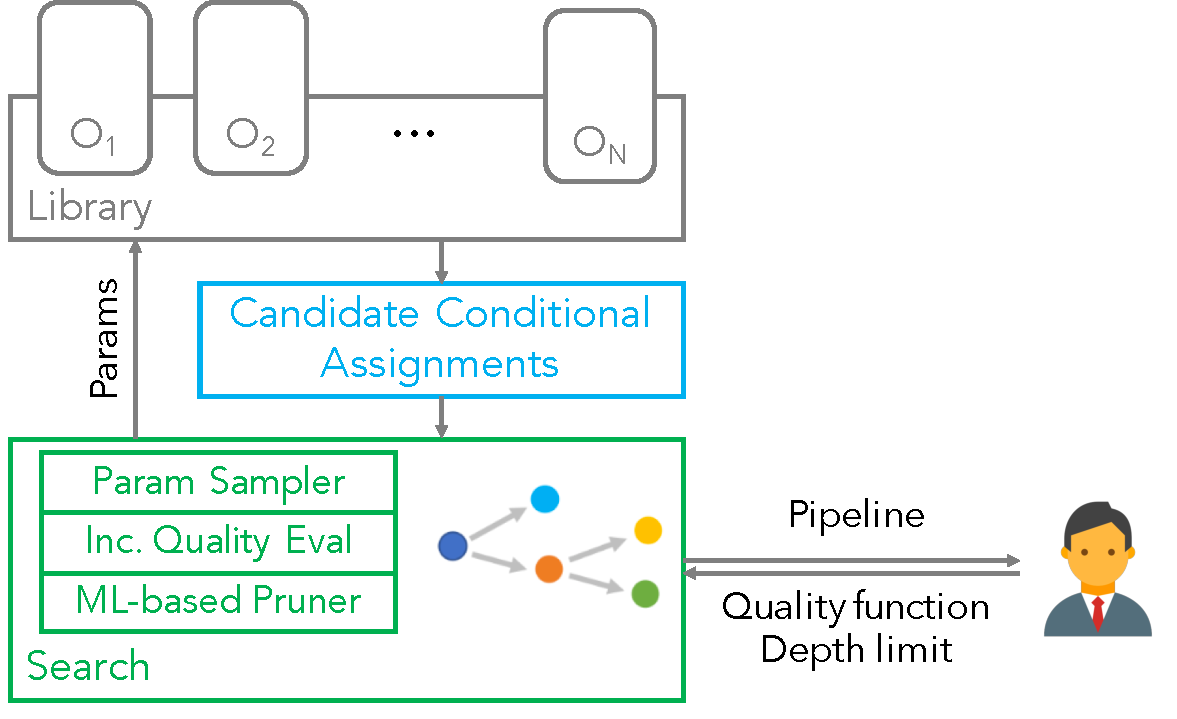
\includegraphics[width=0.7\columnwidth]{figures/arch}
 \caption{\small \sys decouples sampling from the parameter space from search. This allows the user to iterate quickly by observing early best-effort results. \label{fig:arch}}
\end{figure}



\section{Approach Outline}

\sys takes as input a user-provided quality function $Q$, and searches through the space of candidate pipelines $\mathcal{P}$ to find a cleaning pipeline $p^*\in\mathcal{P}$ that maximizes the resulting quality of the relation $Q(p^*(R))$.  \sys is progressive: at any time, \sys reports the best cleaning pipeline found so far.  This helps the user trade-off between search time and cleaning quality.  This section provides an architectural overview, and the following section describes optimizations and implementation details.

% Each conditional assignment can be appended to the current pool of candidate pipelines,  and then extend the current pool of candidate pipelines with the new condi  Thus the cost to execute a given cleaning operator can be an enormous bottleneck on the ability to generate candidate pipelines.  

%The space of possible conditional assignments and cleaning pipelines is far too large, and only a small subset is feasible to materialize at any time. 



\subsection{Naive Synchronous Approach}

Recall that a pipeline is composed of conditional assignments, which are generated by executing cleaning operators with specific parameter values.   A naive approach would select an operator $o$, draw a sample $\phi$ from its parameter space, execute $o(\phi)$ to generate a set of conditional assignments.      It then composes each conditional assignment $ca_i$ to each pipeline $p_j$ in the current pool of candidates, executes the new pipeline $p' = ca_i \circ p$, and evaluates the quality function $Q(p'(R))$.

Blackbox search algorithms typically couple the candidate (condition assignment) generation step with the quality evaluation step, because the former is usually very fast whereas quality evaluation may be slow.  In our context, the opposite is true, and quality evaluation is much faster than candidate generation.   Thus, the naive approach is susceptible to blocking on straggler cleaning operators that take a long time to generate conditional assignments. 

\subsection{Asynchronous Architecture}
We propose a generate-then-search framework, that decouples the execution of cleaning operators and pipeline quality evaluation (Figure~\ref{fig:arch}).  Each operator $O_i$ runs in a separate thread (or process) and continuously reruns $O_i(\phi_k, R)$ with new parameters provided by the {\it Parameter Sampler}.  The {\it Searcher} periodically sends to the Library the output relation $R*$ of the best pipeline so far, and the cleaning operator evaluates over $R^*$.  Its outputs are added to the {\it Conditional Assignments Pool}.  The Searcher removes conditional assignments from this pool to expand the set of candidate cleaning pipelines, and periodically sends the best pipelines so far to the user.   If the pool exceeds a maximum size, it applies back pressure to pause the cleaning operators until the Searcher has removed a sufficient number of conditional assignments the pool.  In practice, the cost to generate candidate assignments is far higher than the search procedure, and back pressure was not needed in our experiments.   The {\it Quality Evaluator} computes the quality of a candidate pipeline, and the {\it ML-based Pruner} prunes the parameter search space using a machine learning model.  Below, we describe the basic implementations of each major component, and describe optimizations in the next Section.


{
\begin{algorithm}[t]
\KwData{Q, R, $\mathcal{P}$, $\gamma$, limit}
// Initialize priority queue of candidate pipelines\\
$S = \{NOOP\}$
\While{limit $> 0$}{
  \For{$s \in S$ }{        
    Pop $s$ from the queue.     
    
    \For{$c \in \mathcal{C}$}{
            $s' = c \circ s$ 
            
            $S.push(s', Q(s'(R)))$
        }    
      $\bar{s} = \argmax_{s\in S} Q(s(R))$\\
      Optional: merge disjoint pipelines (Algorithm~\ref{alg:pruning})
       
      $S= \{s \in S\ |\ s \ge \gamma\times Q(\bar{s}(R)) \}$
    }
    limit -= 1 //decrement limit
  }
\Return Highest priority item on the queue
\caption{Greedy Best-First Tree Search}
\label{alg:main}
\end{algorithm}
}

\stitle{Best-first Search}
Best-first search expands the most promising nodes chosen according to a specified cost function.
\Cref{alg:main} greedily removes nodes on the frontier that are more than $\gamma$ times worse than the current best solution.  Reducing $\gamma$  makes the algorithm asympotically consistent but uses more memory to store the frontier, whereas $\gamma=1$ only keeps the pipelines with the highest quality at every iteration.  

The frontier is modeled as a priority queue $S$ where the priority is the quality of the candidate pipeline, and is initialized with a NOOP operation with the non-transformed dataset quality $Q(R)$ (Line 2).  For each pipeline $s\in S$ (Line 3), we remove each conditional assignment $c\in\mathcal{C}$ that is present at the start of the iteration; conditional assignments added later are processed in a subsequent search iteration.  We compose the pipeline with $c$ and add it to $S$.
Finally, let $\bar{s}$ be the highest quality plans in the queue. Line 11 removes all pipelines whose quality is $<\gamma\times Q(\bar{s}(R))$ from the frontier.  
This process repeats until the candidate pipelines cannot be improved or the pipeline reaches a maximum limit $limit$.


% \ewu{can be cut} Since each plan $s' = c\circ s$ is the composition of a previous candidate pipeline $s$ and a transformation $c$, an obvious optimization is to materialize the output of $s(R)$ and compute $s'(R) = T(s(R))$ as a function over the materialized intermediate relation.  Using the incremental quality function evaluation from Section~\ref{s:qualityivm}, we simply compute the delta between $s'(R)$ and $s(R)$ and incrementally update the quality.


\stitle{Discussion} The key benefit of this asynchronous approach is that the search process does not block on a straggler cleaning operator.  It is common that operator parameters affect their runtime.  For example, inference thresholds and partitioning parameters can have ``cliffs'', where a small change in parameters can drastically slow down the performance of the method. Including such parameter settings in the search process naively would block the entire system.  In contrast, \sys will simply sample from faster operators until the slow inference task completes.    In fact, this design explicitly highlights the connection between the explored search space and resource scheduling.  For instance,  allocating more CPU resources to more promising operators can affect how the search space is explored.

One drawback of the asynchronous approach is that the Parameter Sampler is oblivious of the search process, so the cleaning operators may generate conditional assignments that are not useful.  However, we use this approach because it enables a uniform featurization process over conditional assignment operators, rather than needing to develop custom models for arbitrary cleaning operators.  Further, we find that this approach works well across existing data cleaning benchmarks and use cases.  

To show the power of a general search-based data cleaning system, \sys applies straightforward optimizations but otherwise uses default implementations of the components.  The primary optimizations focus on a parallel implementation of the search algorithm (Section~\ref{s:search}), computing the quality functions incrementally using incremental view maintenance ideas (Section~\ref{s:qualityivm}), and pruning the search space by learning a prediction model (Section~\ref{s:pruning}).  The {\it Parameter Sampler} does not attempt to preferentially sample from ``more promising'' parameter spaces, and simply uses uniform sampling.  Similarly, the Library does not perform resource scheduling, and simply allocates one thread per cleaning operator, and each process executes parameter assignments serially. 


% Our main architectural insight is a generate-then-search framework.  Possible parameter values are fed into a library of data cleaning methods, and these parameter assignments asynchronously generate candidate repairs to the dataset (called conditional assignments).  In parallel, a search thread builds a data cleaning plan using compositions of those transformations in the set.  Existing search algorithms implicitly pipeline these two steps; whereas, we decouple these two steps where candidate repairs can be generated in a separate thread and the search algorithm can proceed independently.  This contrasts from the baseline architecture, hereafter called \emph{synchronous tuning}, where a hyperparameter tuning algorithm will then select and assign parameter values to a sequence of operators and evaluate the quality at the end.  There are a few benefits for the asynchronous architecture of \sys.


% \vspace{0.5em} \noindent \textbf{Benefit 2. Progressive Results: } Next, the decoupling also allows for improved progressive behavior with early results. The search thread continuously polls the candidate conditional assignment set for new expansions. The naturally faster  data cleaning methods (e.g., approximate) will generate candidate repairs faster. Slower methods will eventually add these candidate repairs. This allows users to identify faults or glitches in their quality specifications or parameter spaces more quickly than if all methods were synchronously tuned in a pipeline.
